\begin{title}[\Large]
  Криволинейные интегралы первого рода
\end{title}

\begin{block}[Кривая]
  Кривая это упорядоченное множество точек $\Gamma \subset R^3$

  $\vec \varphi = \vec \varphi(t) = (x(t), y(t), z(t)) ~~~ t = [a,b]$

  $R \to R^3$ непрерывно

  $\vec \varphi(a)$ начальная точка кривой

  $\vec \varphi(b)$ конечная точка кривой

  $\vec \varphi'([a,b]) \not= 0$ тогда гладкая

  Кривая называется кусочно гладкая если каждая ее гладкая часть начинается с
  другой гладкой части (может быть разорвано)

  Если кривая самопересекается то называется не простой иначе простой.

  $\vec \varphi(a) = \vec \varphi(b)$ замкнутая кривая (контур)
  \\

  $\vec \rho = \vec \rho(\tau) = (u(\tau), v(\tau), w(\tau)) ~~
  \tau \in [\alpha, \beta]$

  $\vec \rho$ эквивалентна $\vec \varphi$ если $\exists t(\tau)$
  взаимооднозначное отображение, строго $\nearrow$, $t'(\tau) > 0$ тогда замена
  параметра допустима

  $\vec \rho(\tau) = (x(t(\tau)) = v(\tau), y(t(\tau)) = u(\tau),
  z(t(\tau)) = w(\tau))$
\end{block}

\begin{define}[криволинейного интеграла первого рода]
  $\Gamma \subset R^3$ кривая которая задается с помощью параметрического
  задания $\vec \varphi = \vec \varphi(t) =
  (x(t), y(t), z(t)) ~~ t \in [a,b]$ кусочно-гладкая и $f(x,y,z)$ непрерывна
  на $\Gamma$ тогда
  криволинейным интегралом первого рода от $f(x,y,z)$ на $\Gamma$ называется
  определенный интеграл вида
  $$
  \int_a^b f(x(t), y(t), z(t))|\vec \varphi'(t)|dt =
  $$
  $$
  = \int_a^b f(x(t), y(t), z(t)) \sqrt{x'^2(t) + y'^2(t) + z'^2(t)} dt =
  $$
  $$
  = \int_{\Gamma} f(x,y,z) d l
  $$
\end{define}

\begin{theorem}[проверки коректности определения]
  Криволинейный интеграл 1-ого рода не зависит от способа задания кривой
  $\Gamma$
\end{theorem}

\begin{proof}
  $$
  \int_a^b f(x(t), y(t), z(t))|\vec \varphi'_t(t)|dt =
  \int_{\alpha}^{\beta} f(v(\tau), u(\tau), w(\tau))
  |\vec \rho'_{\tau}(\tau)|d\tau =
  $$
  $$
  = \int_{\alpha}^{\beta} f(x(t(\tau)), y(t(\tau)), z(t(\tau)))
  |\vec \varphi'_t(t(\tau))| t'(\tau)d\tau =
  $$
  $$
  = \int_{\alpha}^{\beta} f(v(\tau), u(\tau), w(\tau))
  |\vec \varphi'_t(t(\tau))| d\tau =
  $$
  $$
  = \int_{\alpha}^{\beta} f(v(\tau), u(\tau), w(\tau))
  |\vec \rho'_{\tau}(t(\tau))| d\tau =
  $$
\end{proof}

\begin{theorem}
  Криволинейный интеграл первого рода не зависит от ориентации кривой $\Gamma$
  $$
  \int_{\Gamma} f(x,y,z) d l = \int_{\Gamma^-} f(x,y,z) d l
  $$
\end{theorem}

\begin{proof}
  $\vec \rho (\tau) = \vec \varphi (a+b-\tau) ~~ \tau \in [a,b]$
  $$
  \int_{\Gamma^-} f(x,y,z) d l = \int_a^b
  f(x(a+b-\tau),y(a+b-\tau),z(a+b-\tau)) |\varphi'_{\tau}(a+b-\tau)|d \tau =
  $$
  $$
  =
  \left|
    \begin{array}{l}
      a+b-\tau = t \\
      dt = -d\tau
    \end{array}
  \right|
  = \int_a^b f(x(t),y(t),z(t))
  |\vec \varphi'_t(t)| dt = \int_{\Gamma} f(x,y,z) dl
  $$
\end{proof}

\begin{theorem}
  $\Gamma$ кусочно гладкая кривая $\Gamma = \Gamma_1 \cup \Gamma_2 \cup
  \ldots \cup \Gamma_m$
  $$
  \int_{\Gamma} f(x,y,z) d l = \sum_{k=1}^m \int_{\Gamma_k} f(x,y,z) d l
  $$
\end{theorem}

\begin{proof}
  Доказательство вытекает из соответствующего свойства определенного интеграла.
\end{proof}

\begin{title}[\Large]
  Криволинейный интеграл второго рода
\end{title}

\begin{define}[плоского поля]
  $(P(x,y,z), Q(x,y,z), R(x,y,z)) = \vec F(x,y,z)$
  векторное поле,
  если можно так выбрать систему координат что $Q$ или $P$ или $R$ $\equiv 0$
  тогда поле плоское.
\end{define}

\begin{define}[криволинейного интеграла второго рода]
  Область $\Omega \subset R^3$ $(P(x,y,z), Q(x,y,z), R(x,y,z)) = \vec F(x,y,z)$
  векторное поле и кусочно гладкая кривая
  $\Gamma \subset \Omega$ $\vec \varphi = \vec \varphi(t) = (x(t), y(t), z(t))
  ~~~ t \in [a,b]$
  криволинейным интегралом второго рода называет определенный интеграл
  $$
  \int_a^b (P(x(t), y(t), z(t))x'(t) + Q (x(t), y(t), z(t))y'(t) +
  R(x(t), y(t), z(t))z'(t))dt =
  $$
  $$
  = \int_{\Gamma} (\vec F, d \vec \varphi) =
  \int_{\Gamma} Pdx + Qdy + Rdz
  $$
\end{define}

\begin{theorem}
  Криволинейный интеграл второго рода не зависит от выбора парамтризации

  $\vec \varphi = \vec \varphi(t) = (x(t), y(t), z(t)) ~~ t \in [a,b]$

  $\vec \rho = \vec \rho(\tau) = (u(\tau), v(\tau), w(\tau)) ~~ \tau \in
  [\alpha, \beta]$
  $$
  \int_{\Gamma} (\vec F, d \vec \varphi) = \int_{\Gamma}(\vec F, d\vec \rho)
  $$
\end{theorem}

\begin{proof}
  $t = t(\tau) ~~~ [\alpha, \beta] \to [a,b] ~~~ t'(\tau) > 0$
  $$
  u(\tau) = x(t(\tau))
  ~~~
  \upsilon(\tau) = y(t(\tau))
  ~~~
  \omega(\tau) = z(t(\tau))
  $$
  $$
  \int_a^b (P(x(t), y(t), z(t))x'(t) + Q (x(t), y(t), z(t))y'(t) +
  R(x(t), y(t), z(t))z'(t))dt =
  $$
  $$
  = \int_{\alpha}^{\beta} (P(u(t), \upsilon(t), \omega(t))u'(t) + Q (u(t),
  \upsilon(t), \omega(t))\upsilon'(t) + R(u(t), \upsilon(t),
  \omega(t))\omega'(t))d\tau
  $$
  $$
  \int_{\alpha}^{\beta} (P(x(t(\tau)), y(t(\tau)), z(t(\tau)))x'_t(t(\tau)) +
  Q (x(t(\tau)), y(t(\tau)), z(t(\tau)))y'_t(t(\tau)) +
  $$
  $$
  + R(x(t(\tau)), y(t(\tau)), z(t(\tau)))z'_t(t(\tau))) t(\tau) d\tau =
  $$
  $$
  = \int_{\alpha}^{\beta} (P(u(t), \upsilon(t), \omega(t))u'(t) + Q (u(t),
  \upsilon(t), \omega(t))\upsilon'(t) + R(u(t), \upsilon(t),
  \omega(t))\omega'(t))d\tau
  $$
\end{proof}

\begin{theorem}
  $$
  \int_{\Gamma^-} (\vec F, d\vec \varphi) = - \int_{\Gamma^+} (\vec F, d \vec
  \varphi)
  $$
\end{theorem}

\begin{proof}
  $\vec \varphi = \vec \varphi(t) = (x(t), y(t), z(t)) ~~ t \in [a,b]$

  $\vec \rho = \vec \rho (\tau) = \vec \varphi(a+b-\tau) ~~ \tau \in [a,b]$
  $$
  \int_{\Gamma^-}(\vec F, d\vec \rho) = \int_a^b (\vec F(u(\tau), v(\tau),
  w(\tau)), d\vec \rho (\tau)) =
  $$
  $$
  = \int_a^b (\vec F(x(a+b-\tau),y(a+b-\tau),z(a+b-\tau)),
  d\vec \varphi(a+b-\tau))
  =
  $$
  $$
  =
  \left|
    \begin{array}{l}
      a+b-\tau = t \\
      dt = -d\tau
    \end{array}
  \right|
  = \int_a^b (\vec F(x(t), y(t), z(t)), (-d\vec \varphi(t)))(-dt) =
  $$
  $$
  = - \int_a^b (\vec F(x,y,z), d \vec \varphi)
  = \int_a^b (\vec F, d \vec \varphi)
  $$
  $$
  d\vec \rho(\tau) = \vec \rho'_{\tau} d\tau = (\vec \varphi'_t, \rho'_{\tau})
  d\tau = -\vec \varphi'_t d\tau
  $$
\end{proof}

\begin{theorem}
  $\Gamma = \Gamma_1 \cup \Gamma_2 \cup \ldots \cup \Gamma_m$ кусочно гладкая
  кривая
  $$
  \int_{\Gamma} (\vec F, d\vec \varphi) = \sum_{k=1}^m \int_{\Gamma_k}
  (\vec F, d\vec \varphi)
  $$
\end{theorem}

\begin{theorem}
  $\Gamma$ плоская кривая $(x,y)$ график $y = f(x) ~~ x \in [a,b]$ тогда
  $$
  \int_{\Gamma} P(x,y)dx = \int_a^b P(x, f(x))dx
  $$
\end{theorem}

\begin{title}[\Large]
  Формула Грина
\end{title}

\begin{define}[односвязаной области]
  $D \subset R^2$ область называется односвязной если $\forall$ замкнутого
  контура $\Gamma \subset D$ ограничена $\partial Q = \Gamma$
  лежит полностью $Q \subset D$

  По колхозному: односвязанная область это область без дырок.
\end{define}

\begin{block}[Формула Грина]
  $D \subset R^2$ односвязанная область в котором задана непрерывно
  дифференцируемое поле $(P,Q)$ тогда $\forall \Gamma \subset D$
  $\Gamma = \partial \Omega$ замкнута и
  ориентация против часовой стрелки
  $$
  \int_{\Gamma} Pdx + Qdy = \iint_{\Omega}  \left( \frac{\partial Q}{\partial x}
  - \frac{\partial P}{\partial y} \right) dxdy
  $$
\end{block}

\begin{proof}
  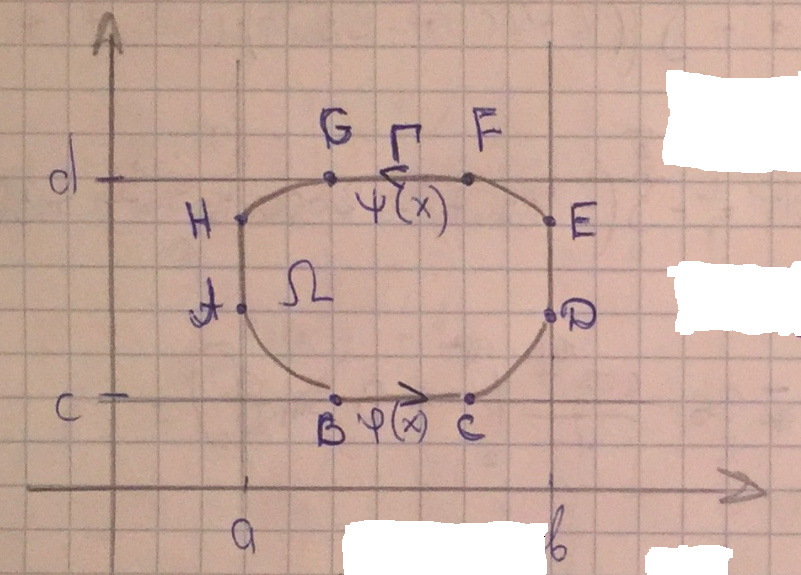
\includegraphics[width = 6cm]{formulaGrin}

  Докажем для $\Omega$ элементарный относительно обеих осей

  1)

  $\Gamma_{ABCD}: y = \varphi(x) ~~ x \in [a,b]$

  $\Gamma_{HGFE}: y = \psi(x) ~~ x \in [a,b]$
  $$
  \iint_{\Omega} \left( -\frac{\partial P}{\partial y} \right) dx dy =
  -\int_a^b dx \int_{\varphi(x)}^{\psi(x)} \frac{\partial P}{\partial y} dy =
  $$
  $$
  = -\int_a^b dx P(x,y) |_{\varphi(x)}^{\psi(x)} =
  - \int_a^b P(x, \psi(x))dx + \int_a^b P(x, \varphi(x)) dx =
  $$
  $$
  = -\int_{\Gamma_{HGFE}} P(x, y) dx + \int_{\Gamma_{ABCD}} P(x,y)dx =
  \int_{\Gamma_{ABCD}} P(x,y)dx + \int_{\Gamma_{EFGH}} P(x,y)dx +
  $$
  $$
  + \int_{\Gamma_{HA}} P(x, y)dx + \int_{\Gamma_{DE}} P(x,y) dx =
  \int_{\Gamma} P(x,y) dx
  $$
  2)

  $\Gamma_{GHAB}: y = \varphi(x) ~~ x \in [a,b]$

  $\Gamma_{CDEF}: y = \psi(x) ~~ x \in [a,b]$
  $$
  \iint_{\Omega} \frac{\partial Q}{\partial x} dx dy =
  \int_c^d dy \int_{\varphi(y)}^{\psi(y)} \frac{\partial Q}{\partial x} dx =
  $$
  $$
  = \int_c^d dy Q(x,y) |_{\varphi(x)}^{\psi(x)} =
  \int_c^d Q(\psi(y), y)dy - \int_c^d Q(\varphi(y), y) dy =
  $$
  $$
  = \int_{\Gamma_{CDEF}} Q(x, y) dy - \int_{\Gamma_{GHAB}} Q(x,y)dy =
  \int_{\Gamma_{CDEF}} Q(x, y) dy + \int_{\Gamma_{BAHG}} Q(x,y)dy +
  $$
  $$
  + \int_{\Gamma_{FG}} Q(x, y)dy + \int_{\Gamma_{BC}} Q(x,y) dy =
  \int_{\Gamma} Q(x,y) dy
  $$
\end{proof}

\begin{title}[\Large]
  Условия независимости криволинейного интеграла 2-ого рода от пути
  интегрирования (плоский случай)
\end{title}

\begin{define}[потенциальности векторного поля]
  Непрерывное векторное поле $(P(x,y), D(x,y))$ называется потенциальным в
  области $D \subset R^2$ если $\exists u = u(x,y)$ (называется потенциалом)
  непрерывно дифференцируема и
  $$
  du = Pdx + Qdy \Leftrightarrow
  \left\{
  \begin{array}{c}
    \frac{\partial u}{\partial x} = P(x, y) \\

    \frac{\partial u}{\partial y} = Q(x, y)
  \end{array}
  \right.
  $$
\end{define}

\begin{theorem}
  $(P(x,y), Q(x,y))$ непрерывное векторное поле в области $D$ (дырки разрешены)
  тогда следующие условия эквивалентны

  a)
  $$
  \forall L \subset D ~~ \int_L Pdx + Qdy = 0
  $$
  b)
  $$
  \int_{L_{AB}} Pdx + Qdy
  $$
  ($L$ - ломанная соеденияющая точки $A$ и $B$ и лежит в $D$)
  он не зависит от характера ломанной (кривой)

  c) Поле $(P, Q)$ в области $D$ потенциальное
\end{theorem}

\begin{proof}
  Докажем так $a \Rightarrow b \Rightarrow c \Rightarrow a$

  1) $a \Rightarrow b$
  $$
  \int_{L_{AB}} Pdx + Qdy = \int_{L_{AB}} Pdx + Qdy ~~ \text{доказать}
  $$
  $$
  \int_L Pdx + Qdy = 0 ~~~ L = L'_{AB} \cup (L''_{AB})^- \Rightarrow
  \int_{L'_{AB}} Pdx + Qdy - \int_{L''_{AB}} Pdx + Qdy = 0
  $$

  2) $b \Rightarrow c$
  $$
  \int_{L_{AB}} Pdx + Qdy = u(x,y)
  $$
  $$
  w(x + x_{\Delta}, y) = \int_{L_{AB} \cup L_{BB_1}} Pdx + Qdy
  $$
  $$
  \lim_{x_{\Delta} \to 0} \frac{1}{x_{\Delta}} (u(x + x_{\Delta}) - u(x,y))
  = \lim_{x_{\Delta} \to 0} \frac{1}{x_{\Delta}} \int_{L_{BB_1}} Pdx + Qdy =
  $$
  $$
  = \lim_{x_{\Delta} \to 0} \frac{1}{x_{\Delta}} \int_{L_{BB_1}} Pdx =
  $$
  $$
  = \lim_{x_{\Delta} \to 0} \frac{1}{x_{\Delta}} \int_x^{x+x_{\Delta}}
  P(t, y)dt =
  $$
  $$
  = \lim_{x_{\Delta} \to 0} \frac{1}{x_{\Delta}} P(x + \theta x_{\Delta}, y)dt
  = P(x,y) ~~ 0 < \theta < 1
  $$

  $$
  \frac{\partial u}{\partial y} = Q(x,y)
  $$
  Доказать самим

  3) $b \Rightarrow c$

  Если поле $(P, Q)$ потенциально в $D$ то $\forall$ кусочно гладкой кривой
  $\Gamma \subset D$
  $$
  \int_{\Gamma} P dx + Q dy = 0
  $$
  В случае когда $\Gamma$ простая кривая (без самопересечений) для простоты
  $$
  \text{если} ~~ \Gamma \subset D
  \left\{
  \begin{array}{l}
    x = x(t) \\
    y = y(t)
  \end{array}
  \right.
  ~~~ t \in [a,b]
  $$
  $$
  \int_{\Gamma} Pdx + Qdy = \int_a^b (P(x(t), y(t)))x'(t) +
  Q(x(t), y(t))y'(t)dt =
  $$
  так как поле потенциально
  $$
  = \int_a^b \left( \frac{\partial u}{\partial x} \cdot
  \frac{\partial x}{\partial t} + \frac{\partial u}{\partial y}
  \frac{\partial y}{\partial t} dt \right) = \int_a^b
  \frac{du(x(t), y(t))}{dt} dt =
  $$
  кривая замкнута $\Rightarrow$ $a$ и $b$ совпадают
  $$
  = u(x(t), y(t))|_a^b = u(x(b), y(b)) - u(x(a), y(a)) = 0
  $$
\end{proof}

\begin{block}[Следствие]
  Для того чтобы криволинейный интеграл 2-ого рода по любой кусочно гладкой
  кривой замкнутой в области $D$ равнялся нулю $\Leftrightarrow$ чтобы он
  равнялся нулю по любой замкнутой ломанной.
\end{block}

\begin{title}[\Large]
  Потенциальные векторные поля в пространстве $R^2$
\end{title}

\begin{block}[Критерий потенциальности плоского векторного поля]
  Для того чтобы непрерывное дифференцируемое векторное поле $(P, Q)$
  было потенциальным в области $D$ необходимо, а в случае когда
  $D$ односвязанно достаточно чтобы
  $$
  \forall (x,y) \in D  ~~~ \frac{\partial P}{\partial y} =
  \frac{\partial Q}{\partial x}
  $$
\end{block}

\begin{proof}
  1) $\Rightarrow$

  Так как поле $(P,Q)$ потенциально то
  $$
  \left\{
  \begin{array}{lcl}
    \frac{\partial u}{\partial x} = P & \to &
    \frac{\partial^2 u}{\partial y \partial x} =
    \frac{\partial P}{\partial y} \\
    \frac{\partial u}{\partial y} = Q & \to &
    \frac{\partial^2 u}{\partial x \partial y} =
    \frac{\partial Q}{\partial x}
  \end{array}
  \right. ~~~ \text{так как $P$ и $Q$ непрерывно дифференцируемы}
  $$
  По теореме о совподающий производных $\Rightarrow$
  $\frac{\partial P}{\partial y} = \frac{\partial Q}{\partial x}$

  2) $\Leftarrow$

  $\forall L \subset D$ простая замкнутая ломанная, $\partial G = L$ граница
  для $G$, $G \subset D$, ориентация кривой навправлена против часовой стрелки
  $$
  \int_{L = \partial G} Pdx + Qdy =
  \iint_G \left( \frac{\partial Q}{\partial x} -
  \frac{\partial P}{\partial y} \right) dx dy = 0
  ~~ \text{так как} ~~
  \frac{\partial P}{\partial y} = \frac{\partial Q}{\partial x}
  $$

  Для ломанной $L$ состоящей из 3-х звеньев не лежащие на одной прямой всё
  выполнено по формуле Грина.

  Если лежат на одной прямой по свойствам интеграла 2-ого рода.

  Для многих звеньев по интдукции.
\end{proof}
